\documentclass[11pt,letterpaper]{article}
\usepackage[lmargin=1in,rmargin=1in,tmargin=1in,bmargin=1in]{geometry}
\usepackage{../style/homework}
\usepackage{../style/commands}
\setbool{quotetype}{true} % True: Side; False: Under
\setbool{hideans}{true} % Student: True; Instructor: False

% -------------------
% Content
% -------------------
\begin{document}

\homework{6: Due 10/05}{I'm fine. It's just that life is pointless and nothing matters and I'm always tired.}{Andy Dwyer, Parks and Recreation}




% plot

	\[
	%\fbox{
	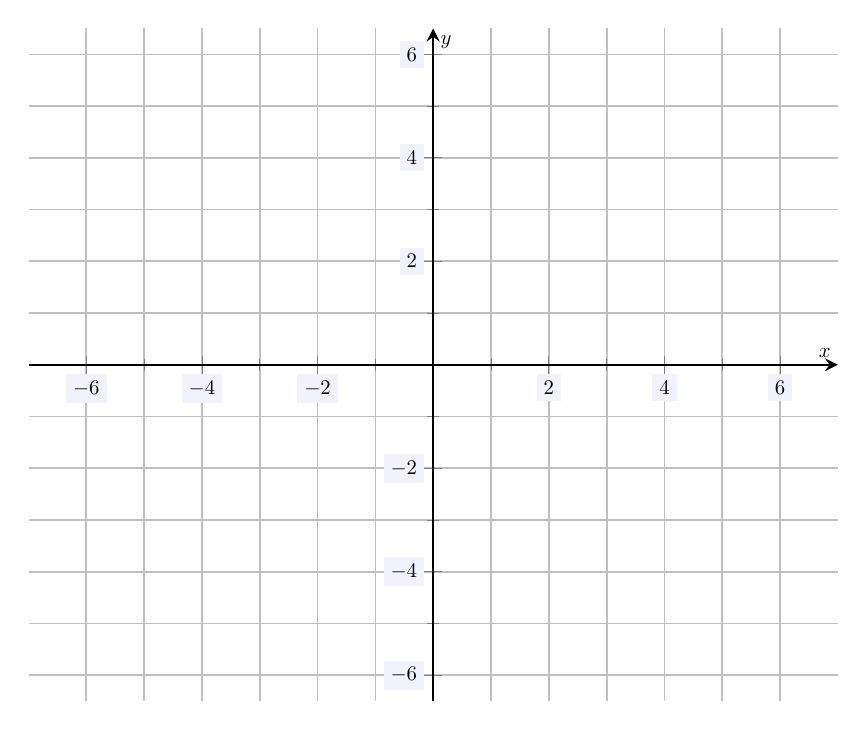
\begin{tikzpicture}[scale=1.5,every node/.style={scale=0.5}]
	\begin{axis}[
	grid=both,
	axis lines=middle,
	ticklabel style={fill=blue!5!white},
	xmin= -7, xmax=7,
	ymin= -6.5, ymax=6.5,
	xtick={-6,-4,-2,0,2,4,6},
	ytick={-6,-4,-2,0,2,4,6},
	minor tick = {-5,-3,...,5},
	xlabel=\(x\),ylabel=\(y\),
%	samples=20
	]

%	\addplot[thick, domain= -7:-3] {-3*x-10};
%	\addplot[thick,domain= -3:2] {4/5*x-3/5};
%	\addplot[thick,domain= 2:4] {7/2*x^2-41/2*x+28};
%	\addplot[thick,domain= 4:7] {2};
%	\addplot[holdot] coordinates{(-3,-1)(2,1)(4,2)};
%	\addplot[soldot] coordinates{(-3,-3)(4,3)};

	\end{axis}
	\end{tikzpicture}
	%}
	\]
% plot
% plot
% point on graph
% point on graph
% even/odd
% avg 
% graph
% graph
% transform













%\printpoints
\end{document}